%
\section{Results and Discussion}

\dave{we should show the nurbs model in rhino/fusion for every example, maybe an exploded view as well}
\dave{mention that not so many standard NURBS models so we modelled lots of these ourselves .. show's power of approach that we can model and sim all these examples.}
\dave{use as many different meshes as possible for figures (i.e try not to have the same mesh show up in more than one figure if possible).}

\begin{table*}[h]
  \caption{Performance of the Shape Matching Element Method on all Examples.}
  \label{tbl:compare}
  \begin{center}
  \begin{tabular}{l c c c c c c c c}
   \textbf{Example} & \textbf{CPU} & $|\vc{q}|$ &  \textbf{Sample Model} & \textbf{Quadrature} & \textbf{Weights} & \textbf{Build $\Pi$} & \textbf{Time Step} \\
   \hline 
   \rowcolor[HTML]{DAE8FC} 
   \textbf{Cantilever}  & ? & ? & ? & ? & ? & ? & ? & ? \\
   \textbf{Rocket}      & ? & ? & ? & ? & ? & ? & ? & ? \\
   \hline
  \end{tabular}
  \end{center}
  
  \end{table*}

%% Results that relate to preprocessing
% weights are good
\begin{figure}
  \centering
  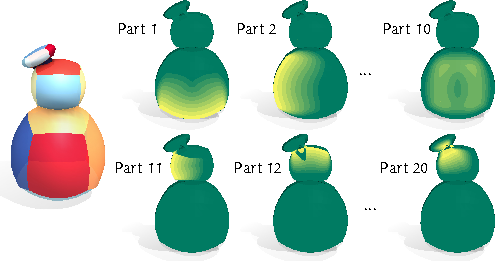
\includegraphics[width=3.33in]{figures/distance_weight_puft.pdf}
  \caption{Our distance weights decay smoothly from 1.0 (yellow) to 0.0 (green) when moving away from its closest surface. Here we visualize the distribution of the distance weights (with cutoff distance 5.0) corresponding to each part.   
  }
  \label{fig:distance_weight_puft}
  \vspace{-5pt}
\end{figure} 
%
%
\begin{figure}
  \centering
  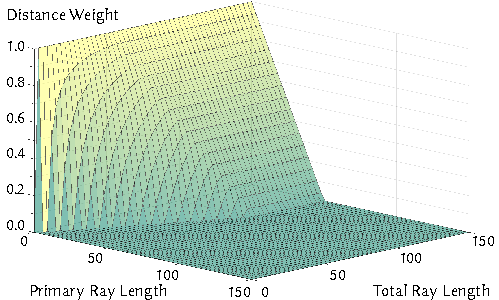
\includegraphics[width=3.33in]{figures/plot_distance_weight.pdf}
  \caption{We plot the distance weight with respect to the primary and total ray length. Here the cutoff distance is 50.
  }
  \label{fig:plot_distance_weight}
  \vspace{-5pt}
\end{figure} 

%kinematic model is expressive
\begin{figure}
  \includegraphics[width=\columnwidth]{example-image-a}
  \caption{Take an intesting geometry (maybe that geometry processing cacture), deform it, do our shape matching and then reconstruct the deformed pose. Do this for a bunch of poses (show's kinematic model is good).}
  \label{fig:deform}
\end{figure}


%% Results that relate to simulation output
%correctness
\begin{figure}
  \includegraphics[width=\columnwidth]{figures/patch_test.pdf}
  \caption{2D examples (left) rigidly transform boundary and show that solving the static problem gives us rigid motion on the interior (right) isotropically scale boundary and show solving static problem gives us constant strain on the interior}
  \label{fig:patchtest}
\end{figure}

\begin{figure}
  \includegraphics[width=\columnwidth]{example-image-a}
  \caption{(left) high res FEM cantileavered bar (right) several simulations using more and more surface patches plus center of mass. Need to show beam is just  unattached patches}
  \label{fig:convergence}
\end{figure}

\begin{figure}
  \includegraphics[width=\columnwidth]{example-image-a}
  \caption{X shape and show arms of X move independently}
  \label{fig:independence}
\end{figure}

% relaxed modeling  constraints
\begin{figure}
  \includegraphics[width=\columnwidth]{figures/mug_overlap}
  \caption{Coffee mug with overlapping handle (top) row of models with increasing overlap (middle) single weight image showing behaviour in the overlapping region, (bottom) simulation result for each one}
  \label{fig:badmodels}
\end{figure}

%different material parameters / material models 
\begin{figure}
  \includegraphics[width=\columnwidth]{example-image-a}
  \caption{Big image simulating the rocket with all different combinations of things}
  \label{fig:materials}
\end{figure}

%different surface reps
\begin{figure}
  \includegraphics[width=\columnwidth]{example-image-a}
  \caption{show subd simulation if we have it. If it works really well we'll just mix subds and nurbs throughout the paper. }
  \label{fig:subd}
\end{figure}

%editing example
\begin{figure}
  \includegraphics[width=\columnwidth]{example-image-a}
  \caption{show input to simulation, show output then show output loaded in rhino/fusion 360 }
  \label{fig:edit}
\end{figure}


%multiple materials
\begin{figure}
  \includegraphics[width=\columnwidth]{example-image-a}
  \caption{Avocado to show heterogenous materials}
  \label{fig:avocado}
\end{figure}

%show stoppers
\begin{figure*}[htp]
  \includegraphics[width=\textwidth,height=3in]{example-image-a}
  \caption{sequence of frames from staypuft simulation}
  \label{fig:staypuft}
\end{figure*}

\begin{figure*}[htp]
  \includegraphics[width=\textwidth,height=3in]{example-image-a}
  \caption{sequence of frames from F1 car simulation}
  \label{fig:f1}
\end{figure*}
